\section{State estimation}
%\subsection{Previous work}
Nevn EKF, unscented particle filter, unscented EKF, classical approach, forskjellige papers som tar for seg deler av det vi ønsker å gjøre, men ikke alt. Nevn også at Automatica08 gjør nesten alt, men ikke gjør bank og inclination estimation, mens MainStateEst gjør alt unntatt yaw rate estimation, så vi ender opp med å snekre sammen begge disse. Nevn også at en del av arbeidet faktisk ikke blir gjort i de to direkte, men i imsland osv. Nevn også at EKF trenger mer tuning og mer beregningskraft. Muligens si det i neste subsubsection som en motivasjon for valg av approach. \\ 

State estimation in general usually referes to the following problem: Given a general nonlinear system 

\begin{equation}
    \Dot{x} = f(x,u(t), w(t))
\end{equation}

where $x$ is the state, $u(t)$ is the input at time $t$ and $w(t)$ is the noise input, and a nonlinear measurement function

\begin{equation}
    y = h(x,v(t))
\end{equation}

where $y$ is the measurement and $v(t)$ is measurement noise. In the specific case met by Revolve NTNU the states we want to approximate are the linear and angular velocities, which are then to be integrated up to give an initial estimate of the position, that is later to be corrected by SLAM. \\

The general field of state estimation is a broad one, that has been studied extensively. Below is detailed some general state estimation algorithms and design methodologies, as well as some that are more specific to our case. Some of the algorithms make more assumptions on the dynamical model, measurement function and the model and measurement noise, and thus it must be evaluated if it fits the specific problem at hand before it is chosen. \\

\subsection{Last years solution}

Last year this problem was solved by a rather rudiemental approach, colored by haste, as the team was scrambling to get everything else up and running for the first Revolve NTNU driverless car. It consisted of only using the RPM measurements from the wheels, taking the mean of them, multiplying with a constant estimate of the wheel radii to get the estimate of forward velocity $v_x$. The yaw rate was approximated by using the difference in the front wheel RPMs and the track width (see figure \ref{Fig:NameOfCarParts}).  \\ 

This very crude approximation gave ok results at very low speeds, but did not work at all at higher speeds, mostly because of wheel slip. The algorithm run on the same track at two different speeds can be seen in figure \ref{Fig:PureWheelOdom}, and clearly illustrates the degradation of performance at anything above very low speeds.   

\subsection{Kalman filter}

One could argue that the Kalman filter is the most widely used and most successfull algorithms to ever come out of the control comunity. It is ubiquitous, showing up in everything from cars to cell phones. What it is at its core is a way of combining sensor data and knowledge of a dynamical system, to get a better estimate of its states, even when faced with noise. \\ 

A kalman filter uses a dynamical model of a system, as well as knowledge of the noise that influences it, and is capable of combining several different types of sensors, making it a very powerfull and easy way of doing sensor fusion. It estimates how the system will develop, propagating not only its states, but also its covariance. This makes it able to know optimally how much it should give weight to measurements compared to the estimates coming out of integrating the dynamical model. \\ 

The kalman filter is said to be the optimal estimator when applied to a linear system, or a system that is linearized around it's true solution. The latter is of course not possible, since if we had the true solution we wouldn't need to estimate the states of the system. It does however mean that if we aren't far away from the solution, it will still be a good estimate. Doing so gives an extended Kalman filter\cite{EKF}, and is what is most used, considering most systems in the real world aren't truly linear systems. \\ 

To be more specific, the Kalman filter consists of a linear or linearized system with a transition matrix for each time step $k$, $F_{k}$, a way of influencing the system through the actuator $u_k$, represented as a matrix $B_{k}$. Together they give the apriori estimate of the state

\begin{equation}
    \hat{x}_{k|k-1} = F_k\hat{x}_{k-1|k-1} + B_k u_k
\end{equation}

To filter this, one propagates the covariance through the system, to find the predicted error covariance

\begin{equation}
    P_{k|k-1} = F_k P_{k-1|k-1} F^T_{k} + Q_k
\end{equation}

where $Q_k$ is the system noise covariance, and $P_{k-1|k-1}$ is the error covariance in the previous step. The error between the measured state $z_k$ and the estimated state $H_k \hat{x}_{k|k-1}$ is then found, where $H_k$ is the linear or linearized measurement function. Call this error $\Tilde{y}_k$. To find the optimal weighting between measurement and estimation, the so called Kalman gain, $K_k$, is created

\begin{equation}
    K_k = P_{k|k-1}H^T_kS^{-1}_k
\end{equation}

where 

\begin{equation}
    S_k = R_k + H_kP_{k|k-1}H^T_k
\end{equation}

is the measurement noise, $R_k$, plus the propagated noise from the previous step. This gain is then used to give a high weight to the measurement when the measurement noise is low and system noise is high, and vice versa. The estimate of the state then is

\begin{equation}
    \hat{x}_{k|k} = \hat{x}_{k|k-1} + K_k\Tilde{y}_k
\end{equation}

To set up for the next step, the a posteriori covariance is found by

\begin{equation}
    P_{k|k} = (I-K_kH_k)P_{k|k-1}(I-K_kH_k)^T + K_kR_kK^T_k
\end{equation}

This gives an error of 

\begin{equation}
    \Tilde{y}_{k|k} = z_k - H_k\hat{x}_{k|k}
\end{equation}

which can be proven to be optimal for linear systems and around the true trajectory of linearized nonlinear systems, as is done in e.g. in the original paper by Rudolf E. Kalman \cite{kalmanOG}.

\subsection{Advanced kalman filters}
There are extensions to the EKF, that gives better properties on some specific problems. One of the most applied of these is the Multiplicative Extended Kalman Filter (MEKF)\cite{MEKF}, and its derivations. It deals specifically with the problem of estimating the states of a 6DOF rotating rigid body in euclidian space. \\ 

The algorithm avoids some of the problems, like singularities, of dealing with attitude in a three-variable parametrization like Euler Yaw, Pitch, Roll, by working on a redundant parametrization for the attitude. This removes the singularities, but makes the state update a little more involved. The MEKF represents attitude as the product of an estimated attitude and the deviation from that attitude. Most implementations use a quaternion representation, leading to a product 

\begin{equation}
    q = \delta q(\phi)\oplus \Hat{q}
\end{equation}

where $\Hat{q}$ is the unit estimated quaternion and $\delta q(\phi)$ is a unit quaternion representing the rotation from $\Hat{q}$ to the actual attitude $q$, here parametrized by a vector, $\phi$, with three components. The choice of $\phi$ might vary, but usually the small angle approximation

\begin{equation}
    \delta q(\phi) = \begin{bmatrix} \phi / 2 \\ 1 \end{bmatrix} + \mathcal{O}(||\phi||^2)
\end{equation}

is used to get the correction on the estimate. The MEKF improves the stability properties of the EKF in attitude estimation by removing some singularities, but there is still room for improvement. A generalized MEKF is thus developed in \cite{GMEKF}, that gives a larger convergence region. \\ 

Another way of avoiding the problems of the three variable parametrization is an Additive Extended Kalman Filter (AEKF), which does the same thing, but through addition of quaternions instead. This has however been proven to be equavivalent to the MEKF\cite{AEKF}, and is thus not discussed further. \\

Yet another extendsion of the EKF is the Unscented EKF\cite{UKF}. Instead of linearizing the nonlinear state transition function to be able to propagate the covariance, like the EKF does, it uses what is called an Unscented Transformation\cite{UTrans}. This means that instead of assuming that the first order approximation to the nonlinear function is good enough and discarding the rest of the information it can give us, it approximates the state probability distribution by a set of discrete points, called Sigma points. These and the mean are then propagated through the full nonlinear state transition function. This gives a new predicted mean and the propagated sigma points are used to approximate a new distribution in the transformed space, usually a Gaussian. \\

The points chosen are carefully picked to perfectly represent the mean and covariance of the original distribution, and thus it is proven to give a third order approximation of the propagated distribution for a nonlinear state transition with additive white noise, compared to only a first order approximation in the EKF. For a nongaussian distribution this method is still correct to the second order.\\ 

One update step of the UKF consists of finding a set of sigma points, $x_{k,i}$, from the original distribution and a set of weights, $w_i$, as follows

\begin{alignat*}{3}
    & x_{k-1,0} &&= \Bar{x_k} \\
    & x_{k-1,i} &&= \Bar{x_k} + (\sqrt{(N+\lambda)P_{x,k}}_i, i &&= 1,...,N \\
    & x_{k-1,i} &&= \Bar{x_k} - (\sqrt{(N+\lambda)P_{x,k}}_{i-N}, i &&=N + 1,...,2N \\
    & w_{k-1,0}^{(m)} &&= \lambda/(N+\Lambda) \\ 
    & w_{k-1,0}^{(c)} &&= \lambda/(N+\lambda) + (1-\alpha^2 + \beta) \\
    & w_{k-1,i}^{(m)} &&= w_{k-1,i}^{(c)} = 1/(2(N+\lambda)), i &&= 1,...,2N
\end{alignat*}

where $\lambda = \alpha^2(N+\kappa) - N$ is a scaling parameter. $\alpha$ determines the spread of the points around the mean and is usually set to a small positive value (e.g. 0.001). $\kappa$ is a secondary scaling parameter which is usually set to 0, and $\beta$ is used to incorporate prior knowledge about the distribution ($\beta=2$ is optimal for the Gaussian distribution). $P_{x,k-1}$ is the covariance of $x$ at time $k-1$, and N is the number of state space dimensions. \\

These points are sent through the nonlinear function, giving a set of new points $y_{k-1,i}$. The new points are then used with the weights to give the new mean and covariance matrix of the new points. 


\begin{equation}
    \Bar{y}_{k-1} \approx \sum_{i=0}^{2N} w_{k,i}^{(m)}y_{k-1,i}
\end{equation}

\begin{equation}
    P_{k-1, yy} \approx \sum_{i=0}^{2N} w_{k,i}^{(c)}(y_{k-1,i} - \Bar{y})(y_{k-1,i} - \Bar{y})^T
\end{equation}

To find the Kalman gain, one also need the covariance of the old state with the new, 
\begin{equation}
    P_{k-1, xy} \approx \sum_{i=0}^{2N} w_{k,i}^{(c)}(x_{k-1,i} - \Bar{x})(y_{k-1,i} - \Bar{y})^T
\end{equation}

and the covariance of the old state with itself,

\begin{equation}
    P_{k-1,xy} \approx \sum_{i=0}^{2N}w_{k,i}^{(c)}(x_i - \Bar{x})(x_i - \Bar{x})^T
\end{equation}

All that remains then is to incorporate measurements. To do this one creates the Kalman gain, $K$, much like with the EKF, and use this to weight between the measurement and the estimate.

\begin{equation}
    K_k = P_{k-1,xy}P_{k-1,yy}^{-1}
\end{equation}

This then gives us the posterior estimated state

\begin{equation}
    x_k = x_{k-1} + K_k(z_k - \Bar{y}_{k-1})
\end{equation}

where $z_k$ is the measured state, $\Bar{y}_{k-1}$ is the a priori estimate of the state and $x_{k-1}$ was the previous a posteriori estimate. To the get new state covariance matrix is then simply

\begin{equation}
    P_k = P_{k-1,xx} - K_kP_{k-1,xy}K_k^T
\end{equation}

Although this seems more complicated, it actually is of the same computational order of magnitude as the EKF, and gives a much better approximation.

\subsection{Particle filter}
Another solution to the state estimation problem is the Particle Filter, first introduced in \cite{ParticleFilter} in 1996, but not made viable before 2000, when resampling was introduced\cite{ParticleResampling}. It attacks the problem of state estimation from the view point that the best estimate of the state could be gotten if we had the probability density function of the state given the inputs, measurements and measurement model. But since this is not something we usually have analytically, it instead approximates it by a discrete set of particles, where the density of the particles in the state space over time will approximate the true pdf. \\

The basic principle of a particle filter is 

\begin{itemize}
    \item pulling samples (usually called particles) from a prior distribution, 
    \item weighting them with how much deviation there is from the true distribution, 
    \item normalizing the weights and then resampling the particles (with replacement) where the probability of sampling a specific particle is its weight. 
\end{itemize}

In a state estimation setting this means starting with N particles, distributed in some manner around the state space (usually uniformly). Then every step, $k$, in the particle filter the particles $\{x_{k-1,i}\}$ are propagated according to the state transition function

\begin{equation}
\forall i, \; \; x_{k,i} = f(x_{k-1,i}, u_k)
\end{equation}

where $u_k$ is the input at that step. Here some have had good results with adding some noise to the propagation, in order to speed up exploration of the state space\cite{ParticleNoise}. The weighting function, $p(z_k|x_{k,i})$, is the probability of observing the measurement, $z_k$, given the state. This function is given by the measurement model for the different sensors. In the case of additive gaussian noise on a single sensor with linear measurement function, this is simply

\begin{align}
    p(z_k| & x_{k-1, j}, u_k) \propto \\
    & exp(-1/2(z_k - Cf(x_{k-1, j}, u_k))^T
    (\Sigma_v + C\Sigma_wC^T)^{-1}(z_k - Cf(x_{k-1, j}, u_k))) \nonumber
\end{align}

Where $\Sigma_v$ is the process noise covariance and $\Sigma_w$ is the measurement noise covariance. \\ 

One can also use more heuristic approaches, like using the euclidian distance as the weighting function, normalized to one. This was employed in the particle filter Revolve NTNU uses for path planning. There the weighting of the different center line hypotheses is a function of the sum of the cones' deviations from the mean track width and has given good results.

\subsection{Visual odometry}

A less classical approach to state estimation is Visual Odometry (VO). It exists in many variants, but the main principle is finding correspondences between successive image frames, using geometric considerations on these points or regions to estimate the relative change in pose between the two frames. This gives the change in pose, which can then be summed to give the pose relative to the initial pose, as well as derivated to get an approximate velocity and angular rate.\\ 

One of the most popular algorithms is SVO\cite{SVO} and more recently its stereo extension SVO 2.0\cite{SVO2}. It finds feature points in the two images using FAST corner detection\cite{FAST} and Edgelets egde detector\cite{Edgelet}. Only the points that can be matched between the images are kept. Around the features a patch of pixels are chosen. These patches are then reprojected from one of the frames into the other to find the pose that minimizes photometric error between the reprojection and the true pixels, se figure \ref{Fig:SVO}. \\

\begin{figure}
    \centering
    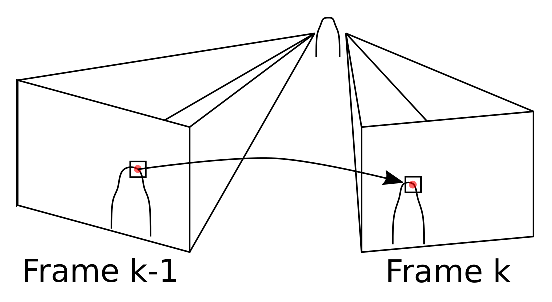
\includegraphics[width=0.8\linewidth]{0_Images/3_Background/SVO.eps}
    \caption[Illustration of SVO's reprojection of an image patch.]
    {Illustration of SVO's reprojection of an image patch. It tries to find the pose that minimizes the photometric error between the pixels projected into the frame and the pixels they get projected onto.}
    \label{Fig:SVO}
\end{figure}

A problem with using one single camera for positioning, is that the two scenes can look identical in the two images, but be of completely different scale. Without stereo information, the camera doesn't give information about scale, thus rendering the positioning information quite useless. This is tackled by either having something in the frame that you know the size of that everything else can relate to, or, as in the case of SVO 2.0, by using two cameras with a known transformation between. This gives gives the scale information needed. \\

SVO and SVO 2.0 are implemented in c++ and publicly available under a non-commercial license. \\

Another viable algorithm is DSO\cite{DSO}. It looks at entire regions of pixels where the pixel intensity gradients are large enough, samples pixels randomly from the regions and tries to find the pose that minimizes the photometric error of the reprojected pixels. \\

The author of the original paper has a publicly available c++ implementation, but although there is a theoretical stereo extension called DSO-Stereo\cite{DSOStereo}, the only implementations of the algorithm that are publicly available is a very unstable one from someone other than the author. \\

Yet another option is ORB-SLAM2\cite{ORBSLAM}, which uses ORB features\cite{ORB} to find point correspondences in two consecutive frames. This gives an initial estimate on the change in position between the frames, as well as distance measurements of different features. It then uses this information to do full SLAM, building a 3D map of points and placing the camera in that map (more on SLAM below). By ignoring the information about the map this is effectively a state estimator as well. ORB-SLAM2 works on a stereo setup and a implementation by the authors is publicly available.

\subsection{Lidar Odometry}

Instead of using the camera information to get a visual odometry, one could apply the same set of ideas to the point cloud coming out of the LiDARs. This gives what is known as LiDAR Odometry. \\ 

The most known, publicly available, algorithm at the moment is LOAM\cite{LOAM}. It, much like ORB-SLAM, finds feature points that it can match in successive swipes of the LiDAR, that then gives point to point distance estimates. These distance estimates are then added iteratively to a set of distances, a single step of a nonlinear optimizer tries to find the pose change between frames. Distance estimates are added untill the optimization step converges. \\

A very recent development is DeepLO\cite{DeepLO}, where they use neural nets, with both supervised and unsupervised training to achieve very good performance on the KITTI dataset. There is however, as of now, no code open to the public.

\subsection{Nonlinear observer}
\iffalse
One of the first papers to treat nonlinear observer design by errorlinearization was \cite{FirstErrorLinNonlinObs}. \\

The first type that should be mentioned is EKF, statisctically motivated. \\ 

Explain the general problem, maybe mentioning stuff like observability, different forms of stability of the observers and especially the convergence to the true value over time. \\

Different types of nonlinear observers that are benefitial to mention

\begin{itemize}
    \item Observers derived by linear approximation (maybe EKF first?)
    \item Statistically motivated expanded degree observers like EKF
    \item Observers derived by error linearization
    \item High gain observers
    \item Minimum energy?
    \item Sliding mode observers?
    \item Before arriving at the main one: Observers derived through Lyapunov analysis
\end{itemize}
\fi

The term nonlinear observer refers to any dynamical system run in parallel with a dynamical system, where some or all of the internal states of the nonlinear observer tries to match some or all the states of the original dynamical system. There are mountains of different nonlinear observers, as this is a very general term. \\ 

To separate the different types of observers, it is benefitial to do so by how they have been derived. This makes it possible to talk about each class' general properties, their pros and cons, especially in regards to ease of derivation for a specific system, how much tuning there is and overall performance.

\subsubsection{Linear approximation}

The first that should be mentioned is the nonlinear observers derived by linear approximation of the dynamical system it is trying to represent\cite{LinearizingNonlinObs}. If this is done for a linear system 

\begin{align}
    \Dot{x} &= Ax + Bu \\
    y &= Cx
\end{align}

the resulting observer

\begin{align}
    \Dot{\hat{x}} &= A\hat{x} + Bu + L(y - \hat{y}) \\
    \hat{y} &= C\hat{x}
\end{align}

will give exponential convergence of the estimate, $\hat{x}$, to the true state, $x$, as long as $A-LC$ is Hurwitz\cite{Hurwitz}. In the case of a nonlinear system the A's, B's and C's will be the first order approximations

\begin{equation}
    A = \frac{\partial f}{\partial x}|_{x=x_0}
\end{equation}
\begin{equation}
    B = \frac{\partial f}{\partial u}|_{x=x_0}
\end{equation}
\begin{equation}
    C = \frac{\partial h}{\partial x}|_{x=x_0}
\end{equation}

where again $f$ is the state transition function and $h$ is the measurement function. This will however only give local asymptotic stability when the $A-LC$ is Hurwitz and the pair $\{A,C\}$ is observable. Many of the relevant dynamical systems do not have this property, nor is local asymptotic stability always enough, so the research community searched on for more sophisticated solutions with better properties. 

\iffalse
One of the next steps the community took was to develop the statistically motivated methods, most prominent and succesfull of which is the Extended Kalman filter. These methods are typically so-called expanded order observers, meaning they have more internal states than the system that it is trying to approximate the states of. In the case of the Kalman filter these internal states are $\{\hat{x},P\}$, which illustrates usual approach taken by these methods; to approximate not only the state of the system, but also the underlying probability distribution it comes from. 
\fi

\subsubsection{Error linearization}

A rather large theoretical step forward was taken by Krener and Isidori\cite{FirstErrorLinNonlinObs}, when they developed a nonlinear observer by so-called error linearization. The idea is to find transformations of the state and output coordinates, 

\begin{equation}
    z = \Theta(x)
\end{equation}
\begin{equation}
    w = \gamma(y)
\end{equation}

such that nonlinear system can be expressed in the form

\begin{align}
    \Dot{z} &= Az + \alpha(u,y) \\
    w &= Cz + \beta(u,y)
\end{align}

This makes it easy to make an observer for the system

\begin{align}
    \Dot{\hat{z}} &= A\hat{z} + \alpha(u,y) + L(w-\hat{w}) \\
    \hat{w} &= C\hat{z} + \beta(u,y) \\
    \hat{z}(0) &= \Theta(\hat{x}^0) \\ 
    \hat{x} &= \Theta^{-1}(\hat{z})
\end{align}

If the pair $\{C,A\}$ is observable and one has placed the spectrum of $A-LC$ in the open left half plane, then this observer will converge exponentially. \\

The problem is of course that not many systems are possible to transform like this, and many who do can only be transformed into this form by repeated derivations of the output. The latter makes the whole design very vulnerable to noise, in fact so much that it has little practical use. \\

\iffalse
A similar approach is the so called High Gain Observer\cite{HighGain}, which gets the system into the uniformly observable form, and then adds a error term of $L(y-\hat{y})$ to each state. If the gain is large enough this can be proven to be locally asympotically stable, but it suffers from the same problems as the error linearization. \\
\fi

\subsubsection{Nonlinear observers designed using Lyapunov analysis}

A more recent developement, spearheaded in part by the research community here at NTNU, is the use of Lyapunov anaysis to develop nonlinear observers that converge asymptotically to the true state\cite{PassiveFossen}. Made first for Dynamic Positioning (DP) of large boats, it consists of starting out with an initial guess for an observer, then trying to prove it's stability by Lyapunov analysis and then modifying the observer until stability can be proven. \\

By Lyapunov analysis\cite{Lyapunov} is meant the process of finding a Lyapunov function candidate $V(\Tilde{x})$ that is positive definite, i.e. larger than or equal to zero for all $x\neq \Vec{0}$. Here $\Tilde{x}$ is the error between the true state and the estimate. The proof is then to show that this function has the special property that

\begin{equation}
    \frac{dt V(\Tilde{x})}{dt} \leq 0 \;\; \forall \hat{x}
\end{equation}

If such a Lyapunov function can be found and this property holds, then the error will always go asymptotically to zero and the observers works as desired. Other properties as also possible to derive with slight changes to the analysis formulation, but this is the main way it is used. \todo{Double check math here and consider rewriting} \todo{Maybe add parts about I/O stability proofs and GES?}. \\

One of the main reasons for choosing a nonlinear observer over a Kalman filter is that once the observer is developed it needs much less tuning than the Kalman filter. An example is the 120 covariance equations in the Kalman filter for the supply vessel discussed in \cite{PassiveFossen}, compared to the 17 gains in the nonlinear observer. Another huge benefit compared to the EKF is global asymptotic stability and sometimes global exponential stability, compared to only local symptotic stability of the EKF. \\ 

For a system of the form 

\begin{align}
    \Dot{x} &= f(x,u,v) \\
    y &= h(x,u,w)
\end{align}

where $x$ is the state, $u$ is the input and $v$ and $w$ are noice inputs, a good place to start for the observer design would be to simply copy the dynamics with a proportional error term, setting the noise to zero.

\begin{align}
    \Dot{\hat{x}} &= f(\hat{x}, u, 0) + K\Tilde{y} \\
    \hat{y} &= h(\hat{x}, u, 0)
\end{align}

Here $\Tilde{y} = y -  \hat{y}$ is the difference between the measured y and the estimated y. A first guess for the Lyapunov function could then be the difference in physical energy of the system when in the true state and when in the estimated state, or the quadratic sum of the error in the estimated states. 